\chapter{Resultados}\label{cap:Resultados}
A partir dos algoritmos implementados na biblioteca \textit{Komm}, foram realizados testes de compressão e descompressão com diferentes conjuntos de dados. Este capítulo apresenta os resultados obtidos, incluindo análises de desempenho e comparações com outras bibliotecas populares encontradas no github.

Para esta secção, foram utilizados 2 tipos de arquivos: arquivos de texto e arquivos de imagem. Os arquivos de texto foram escolhidos por serem comuns em aplicações de compressão, enquanto os arquivos de imagem foram selecionados para avaliar o desempenho.
Os arquivos utilizados foram:
\begin{itemize}
    \item \textbf{Arquivos de Texto:} Alice’s Adventures in Wonderland
    \item \textbf{Arquivos de Imagem:} Imagens no formato bitmap (BMP)
\end{itemize}
O arquivo de texto utilizado foi o livro "Alice’s Adventures in Wonderland", disponível no projeto Gutenberg\footnote{https://www.gutenberg.org/ebooks/11}. Este arquivo é representativo de textos literários e possui uma variedade de caracteres e padrões que são úteis para testar algoritmos de compressão.
As imagens no formatos .bmp podem ser vizuliadas na Figura \ref{fig:smiley} e \ref{fig:snail}.

\begin{figure}[h]
	\centering
	\caption{Imagem no formato bitmap (BMP) de um smiley}
	\label{fig:smiley}
	
\includegraphics[width=5cm]{figuras/smiley-large.png}
    \fonte{https://cse1.net/recaps/graphics}
\end{figure}

\begin{figure}[h]
	\centering
	\caption{Imagem no formato bitmap (BMP) de um caracol}
	\label{fig:snail}
	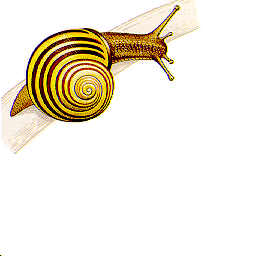
\includegraphics[width=5cm]{figuras/snail.png}
    \fonte{Elaborada pelo autor}
\end{figure}

\pagebreak
\section{Métricas de Avaliação}
Para avaliar o desempenho dos algoritmos de compressão implementados na biblioteca \textit{Komm}, foram utilizadas as seguintes métricas:
\begin{itemize}
    \item \textbf{Taxa de Compressão:} A taxa de compressão é definida como a razão entre o tamanho do arquivo original e o tamanho do arquivo comprimido. Uma taxa de compressão maior indica uma melhor eficiência do algoritmo.
    \item \textbf{Tempo de Compressão e Descompressão:} O tempo gasto para comprimir e descomprimir os arquivos também foi medido. Tempos menores indicam um desempenho melhor do algoritmo.
    \item \textbf{Utilização de Memória:} A quantidade de memória utilizada durante o processo de compressão e descompressão foi monitorada para avaliar a eficiência do algoritmo em termos de recursos computacionais.
    \item \textbf{Integridade dos arquivos: } Após a descompressão, os arquivos foram comparados com os arquivos originais para garantir que não houve perda de dados durante o processo de compressão e descompressão.
\end{itemize}

\section{Resultados Obtidos}
Os testes foram realizados de 2 formas: utilizando apenas o algoritmos encontrados na biblioteca \textit{Komm} e depois um comparativo de desempenho com outras bibliotecas populares encontradas no github. As bibliotecas escolhidas para comparação foram:
\begin{itemize}
    \item \textbf{LZ77-Compressor\footcite{https://github.com/manassra/LZ77-Compressor}:} Uma implementação simplificada do algoritmo de compressão LZ77 em python.
    \item \textbf{FastLZ\footcite{https://github.com/ariya/FastLZ}:} Uma biblioteca de algoritmos de compressão rápida e sem perdas escrita em C.
\end{itemize}

%______________________________________________________________________________________________________________________________________________________________________
% Teste de texto a partir daqui
%______________________________________________________________________________________________________________________________________________________________________

\subsection{Resultados com a biblioteca \textit{Komm}}

Os testes começaram com as implementações disponíveis na \textit{Komm}. 
Testando primeiro a compressão do arquivo de texto \textit{Alice} e posteriormente com uma imagem BMP simples \textit{smiley}, mostrada anteriormente.

As figuras \ref{fig:fig:komm-alice-compression}, \ref{fig:fig:komm-alice-memory} e \ref{fig:fig:komm-alice-time} mostram os resultados obtidos com o arquivo de texto \textit{Alice}, a taxa de compressão, o tempo e o consumo de memória das implementações disponíveis na \textit{Komm} (Huffman, Shannon--Fano, Tunstall, LZ78, LZW e LZ77 com diferentes janelas). Observa-se que:
\begin{itemize}
  \item As variantes do \textit{LZ77} na \textit{Komm} mostram \textit{trade-offs} previsíveis: janelas maiores tendem a melhorar a taxa (menor \% do original), às custas de tempo e memória.
  \item \textit{Huffman} e \textit{Shannon--Fano} são muito rápidos e usam pouca memória, com taxa típica de códigos prefixos estáticos; \textit{Tunstall} usa substancialmente mais memória (dicionários maiores), com custo de tempo correspondente.
  \item \textit{LZ78} e \textit{LZW} ficam entre os extremos em taxa e tempo, como esperado para dicionários construídos \textit{on-the-fly}.
\end{itemize}


\begin{figure}[h]
	\centering
	\caption{Taxa de compressão do texto \textit{Alice} utilizando a biblioteca \textit{Komm}}
	\label{fig:fig:komm-alice-compression}
	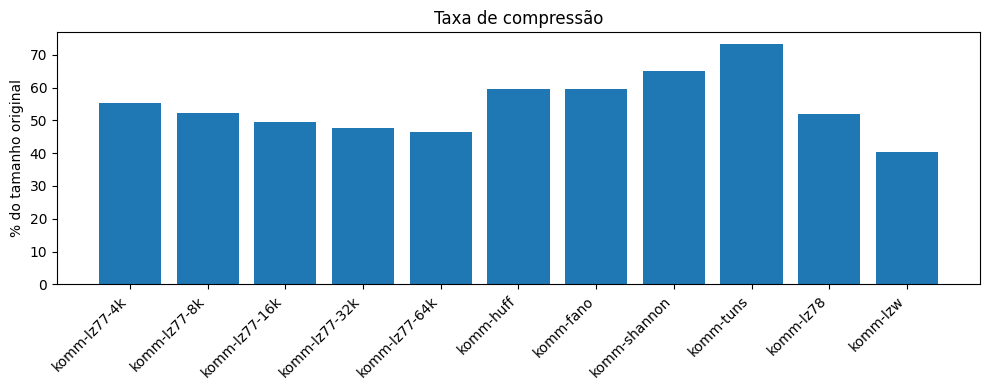
\includegraphics[width=15cm]{figuras/komm_alice_compression.png}
    \fonte{Elaborada pelo autor}
\end{figure}

\begin{figure}[h]
	\centering
	\caption{Uso de memória durante a compressão do texto \textit{Alice} utilizando a biblioteca \textit{Komm}}
	\label{fig:fig:komm-alice-memory}
	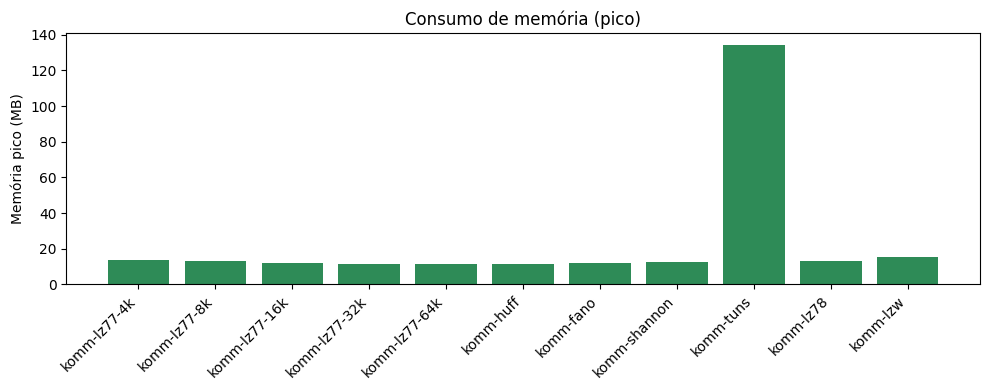
\includegraphics[width=15cm]{figuras/komm_alice_memory.png}
    \fonte{Elaborada pelo autor}
\end{figure}

\begin{figure}[h]
	\centering
	\caption{Tempo de compressão do texto \textit{Alice} utilizando a biblioteca \textit{Komm}}
	\label{fig:fig:komm-alice-time}
	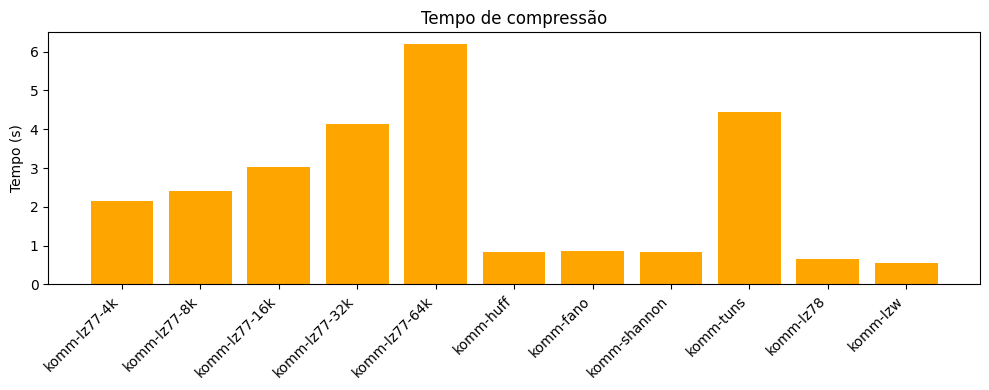
\includegraphics[width=15cm]{figuras/komm_alice_time.png}
    \fonte{Elaborada pelo autor}
\end{figure}

\begin{itemize}
  \item Em imagens com grandes áreas uniformes, o LZ77 se beneficia claramente de janelas maiores (mais chance de reaproveitar repetições longas).
  \item O custo de tempo/memória cresce com a janela, mas permanece estável para os demais algoritmos.
\end{itemize}

\begin{figure}[h]
	\centering
	\caption{Taxa de compressão da imagem \textit{Smiley} utilizando a biblioteca \textit{Komm}}
	\label{fig:fig:komm-smiley-compression}
	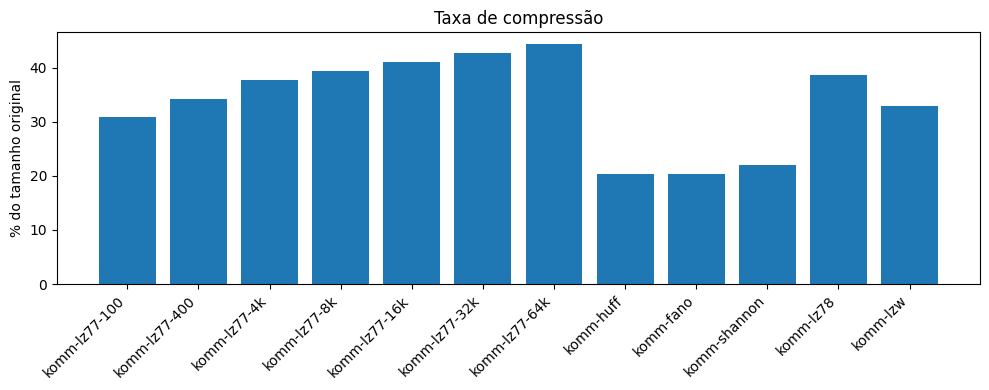
\includegraphics[width=15cm]{figuras/komm_smiley_compression.png}
    \fonte{Elaborada pelo autor}
\end{figure}

\begin{figure}[h]
	\centering
	\caption{Uso de memória durante a compressão da imagem \textit{smiley} utilizando a biblioteca \textit{Komm}}
	\label{fig:fig:komm-smiley-memory}
	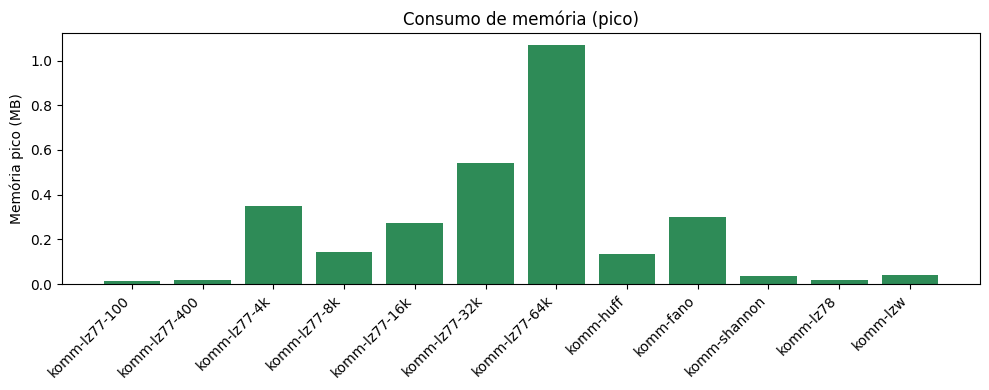
\includegraphics[width=15cm]{figuras/komm_smiley_memory.png}
    \fonte{Elaborada pelo autor}
\end{figure}

\begin{figure}[ht]
	\centering
	\caption{Tempo de compressão da imagem\textit{smiley} utilizando a biblioteca \textit{Komm}}
	\label{fig:fig:komm-smiley-time}
	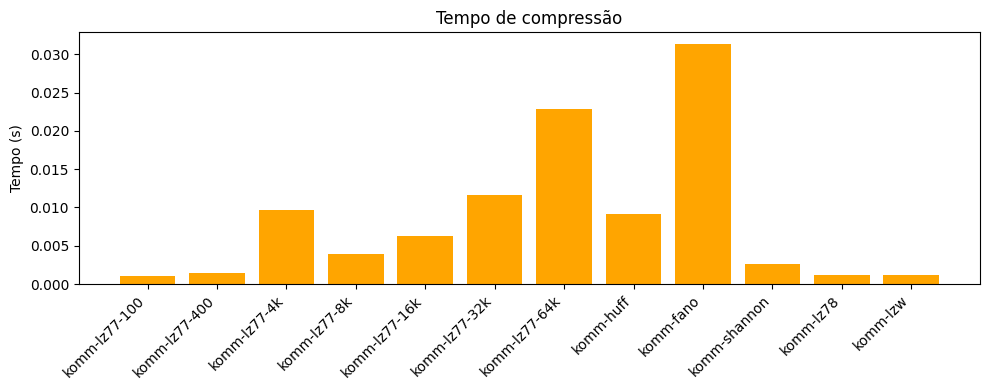
\includegraphics[width=15cm]{figuras/komm_smiley_time.png}
    \fonte{Elaborada pelo autor}
\end{figure}

Para melhor visualização dos dados obtidos com as imagens \textit{smiley}, o Quadro \ref{quadro:resultados-komm-smiley} sumariza os resultados de tempo e uso de memória para os algoritmos testados na \textit{Komm}.

\begin{quadro}[ht]
\caption{Quadro mostrando uso de memoria e tempo dos algoritmos}\label{quadro:resultados-komm-smiley}
\begin{tabular}{|l|r|r|}
    \hline
    \textbf{Algoritmo de compressão}& \textbf{Tempo (s)}  & \textbf{Pico de Memoria (MB)} \\ \hline
    komm-lz77-4k & 0,0096 & 367,894 \\ \hline
    komm-lz77-8k,97 & 0,0039 & 148,218 \\ \hline
    komm-lz77-16k & 0,0062 & 287,370 \\ \hline
    komm-lz77-32k & 0,0115 & 566,106 \\ \hline
    komm-lz77-64k & 0,0228 & 112,2954 \\ \hline
    komm-huff & 0,0092 & 140,961 \\ \hline
    komm-fano & 0,0313 & 314,210 \\ \hline
    komm-shannon & 0,0026 & 38,195 \\ \hline
    komm-tuns & 3,750 & 15.1985,336 \\ \hline
    komm-lz78 & 0,0011 & 19,928 \\ \hline
    komm-lzw & 0,0011 & 43,084 \\ \hline

\end{tabular}
\fonteproprioautor
\end{quadro}

\newpage

\subsection{Resultados obtidos em comparação com códigos externos}

Os testes foram repetidos utilizando as bibliotecas externas \textit{LZ77-Compressor} e \textit{FastLZ}, conforme descrito anteriormente. As figuras \ref{fig:fig:external-alice-compression}, \ref{fig:fig:external-alice-memory} e \ref{fig:fig:external-alice-time} mostram os resultados obtidos com o arquivo de texto \textit{Alice}, a taxa de compressão, o tempo e o consumo de memória das implementações externas comparadas com a melhor implementação da \textit{Komm} (LZ77 com janela de 64kB). Observa-se que:
\begin{itemize}
  \item A implementação externa \textit{FastLZ} apresenta a melhor taxa de compressão, seguida pela \textit{Komm} com LZ77-64kB.
  \item Em termos de tempo, a \textit{Komm} com LZ77-64kB é a mais rápida, seguida pela \textit{LZ77-Compressor}.
  \item A utilização de memória é maior na \textit{FastLZ}, seguida pela \textit{Komm} com LZ77-64kB.
\end{itemize}

\begin{figure}[h]
  \centering
  \caption{Taxa de compressão do texto \textit{Alice} utilizando bibliotecas externas}
  \label{fig:fig:external-alice-compression}
  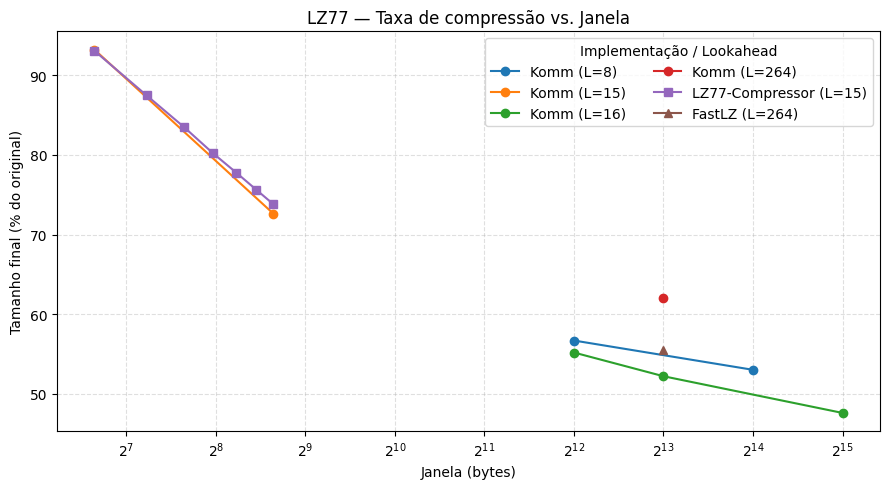
\includegraphics[width=15cm]{figuras/lz77_alice_compression_window.png}
    \fonte{Elaborada pelo autor}
\end{figure}
